\documentclass[a4paper]{article}

\usepackage{amsmath}
\usepackage{amssymb}
\usepackage{stellar}
\usepackage{parskip}
\usepackage{fullpage}
\usepackage{wrapfig}
\usepackage{tikz}

\usetikzlibrary{arrows}
\usetikzlibrary{decorations.pathreplacing}

\title{Fisica I}
\author{Paolo Bettelini}
\date{}

% Integral command
\ExplSyntaxOn
\DeclareDocumentCommand{\integral}{d[] d[] d[] d[]}
{
    \IfNoValueTF { #4 }
    {
        \IfNoValueTF { #3 }
        { \int #1\,d#2 }
        { \text{Either\,\,2\,\,or\,\,4\,\,arguments\,\,must\,\,be\,\,passed} }
    }
    {
        \int\limits\c_math_subscript_token{#1}^{#2} #3 \,d#4
        % In Expl Syntax characters as '_' or ':' are used as letters in command names
        % hence the \c_math_subscript_token{#1} rather than _{#1}
    }
}
\ExplSyntaxOff

\begin{document}

\maketitle
\tableofcontents

\pagebreak

\section{Prodotti vettoriali}

Il prodotto scalare ha lo stesos risultato in ogni base ortonormata

\sproposition{Proprietà del prodotto vettoriale}{
    \begin{enumerate}
        \item \(\vec{a} \wedge \vec{b} = - \vec{b} \wedge \vec{a}\);
        \item \((\gamma \vec{a}) \wedge \vec{b} = \gamma (\vec{a} \wedge \vec{b})\);
        \item \((\vec{a} + \vec{b}) \wedge \vec{c} = \vec{a} \wedge \vec{c} + \vec{b} \wedge \vec{c}\)
    \end{enumerate}
}

Consideriamo \(\vec{a}\) e \(\vec{b}\), allora
\begin{align*}
    \vec{a} &= a_x\hat{x} + a_y\hat{y} + a_y\hat{z} \\
    \vec{b} &= b_x\hat{x} + b_y\hat{y} + b_y\hat{z}
\end{align*}
Sapendo che
\begin{align*}
    \hat{x} \wedge \hat{y} &= \hat{z} \\ 
    \hat{x} \wedge \hat{z} &= -\hat{y} \\
    \hat{y} \wedge \hat{z} &= \hat{x} \\
\end{align*}
Possiamo eseguire il prodotto esplicitamente
\begin{align*}
    \vec{a} \wedge \vec{b} &= a_xb_y\hat{z} + a_xb_z(-\hat{y}) + a_yb_x(-\hat{z})
    + a_yb_z\hat{x} + a_zb_x\hat{y} + a_zb_y(-\hat{x}) \\
    &= \left[a_yb_z - a_zb_z\right] \hat{x} + \left[a_zb_x - a_xb_z\right]\hat{y}
    + \left[a_xb_y - a_yb_x\right] \hat{z}
\end{align*}

\section{Forze apparenti}

Nel caso della terra, la forza di Coriolis è data da
\[
    \vec{F}_c = -m\vec{\omega} \wedge (\vec{\omega} \wedge \vec{r})
\]
È sempre ortogonale all'asse di rotazione (l'equatore).
Il suo modulo è dato da
\[
    F_c = m\omega^2 R \sin\alpha
\]
dove \(\alpha\) è l'angolo compreso e \(R\) il raggio della terra.
La componente verticale è \(m \omega^2 R \sin^2\alpha\).

\pagebreak

\section{Velocità areolare}

Trovare l'equazione del pendolo usando il momento angolare.

\section{Problema dei due corpi}

Sappiamo che \(\vec{F_{12}} = m_1\vec{a_1}\), \(\vec{F_{21}} = m_2\vec{a_2}\)
e che \(\vec{F_{12}} = -\vec{F_{21}}\).
Sappiamo anche che
\[
    \frac{d\vec{Q}}{dt} = m_1\vec{a_1} + m_2\vec{a_2} =\vec{F_{12}} + \vec{F_{21}} = 0
\]
quindi la quantità di moto si conserva.
Adesso scriviamo
\[
    \vec{a_1} - \vec{a_2} - \frac{\vec{F_{12}}}{m_1}
    - \frac{\vec{F_{21}}}{m_2} = \vec{F_{12}} \left(\frac{1}{m_1} + \frac{1}{m_2}\right)
\]
Definiamo la massa ridotta come
\[
    \frac{1}{\mu} = \frac{1}{m_1} + \frac{1}{m_2}
\]
quindi
\[
    \mu(\vec{a_1} - \vec{a_2}) = \vec{F_{12}}
\]
Troviamo allora che
\[
    \vec{a_1} = \frac{d\vec{v_1}}{dt} = \frac{d^2 \vec{r_1}}{dt^2}
\]
e
\[
    \vec{a_2} = \frac{d\vec{v_2}}{dt} = \frac{d^2 \vec{r_2}}{dt^2}
\]
Assieme abbiamo
\[
    \vec{a_1} - \vec{a_2} = \frac{d^2 \vec{r_1}}{dt^2} - \frac{d^2 \vec{r_2}}{dt^2}
    = \frac{d^2}{dt^2} \left(\vec{r_1} - \vec{r_2}\right)
\]
è l'accelerazione della particella 1 vista dalla 2.
È come se fosse la seconda legge di Newton vista da un osservatore posizionato sulla particella 2.
La differenza, è che l'osservatore due darebbe \(\mu\) come massa al posto di \(m_1\).
Anche se lui non può usare le equazioni di Newton, lo fa lo stesso con solamente l'avvertenza di cambiare
la massa, ottenendo comunque qualcosa di corretto.
Più la differenza di masse è grande, più \(\mu\) corrisponde alla massa vera.

\section{Flussi}

Il flusso in un campo di forza è definito come \(f_i = \vec{F} \cdot \vec{n} dA\)
dove va definito l'orientamento del vettore normale \(\vec{n}\).
Per tutta la superficie chiusa il flusso è \(\sum_i f_i\).

\stheorem{Teorema del flusso di Gauss}{
    Il teorema di Gauss dice che se la forza \(\vec{F}(\vec{r}) = \frac{K}{r^2} \hat{r}\),
    allora il flusso sulla superficie chiusa è dato da
    \[
        4\pi K
    \]
    dove la sorgente è interna alla superficie, altrimenti il flusso è zero.
}

\sexample{Se ci trovassimo sul fondo di un buco sulla superficie terrestre
profondo \(R-r\), quale gravità misureremmo?}{
    Dobbiamo considerare la distribuzione della massa, cioè la densità
    \(\rho\) che è approssimativamente omogenea
    \[
        \rho = \frac{3M}{4\pi R^3}
    \]
    Possiamo immaginarci infinite sorgenti che esercitano su di noi una forza
    \[
        \vec{F}(\vec{r}) = - \sum_i G \frac{m \cdot dm_i}{r_i^2}\hat{r_i}
    \]
    Quindi il flusso è dato dalla somma
    \[
        \sum_i -G m \cdot dm_i = -4\pi G m M 
    \]
    Noriamo che per calcolare il flusso dobbiamo fare
    \[
        \sum_i (dS_i) \vec{F_i} \cdot \hat{n_i} = F \sum_i (dS_i) = 4F\pi r^2
    \]
    dove \(\hat{n_i}\) è la normale. Quindi, la forza è data
    \begin{align*}
        F \cdot 4 \pi r &= - gm \cdot 4 \pi \left(\frac{4}{3} \pi r^3\right) \rho \\
        F &= -G\frac{mM}{R^2} \left(\frac{r}{R}\right)
    \end{align*}
    È importante notare che per fare ciò abbiamo considerato le sorgenti
    della massa del volume racchiuso dalla superficie indotta dal punto in cui mi trovo (una sottosfera).
    Le superfici esterne non contribuiscono sempre per il teorema di Gauss.
}

\pagebreak

\section{Derivazione delle leggi di Kepler dalla legge di gravitazione universale}

Consideriamo il sistema Terra-Sole.
Possiamo scrivere le equazioni di Newton per la Terra, sul sistema di riferimento
non inerziale del sole, se alla terra associamo la massa ridotta
\[
    \mu = \frac{M_S M_T}{M_S + M_T}
\]
Quindi
\begin{align*}
    \mu \frac{d^2\vec{r}}{dt^2} &= - G \frac{M_S M_T}{r^2} \hat{r} \\
    \frac{M_S M_T}{M_S + M_T} \frac{d^2\vec{r}}{dt^2} &= - G \frac{M_S M_T}{r^2} \hat{r} \\
    \frac{d^2\vec{r}}{dt^2} &= - G \frac{M_S + M_T}{r^2} \hat{r}
\end{align*}
che è l'equazione che avrei scritto se avessi considerato un sistema
con un oggetto di massa \(M_S + M_T\).

Ricordiamo che vi sono delle proprietà che vengono conservate, come
\[
    \vec{L} = \vec{r} \wedge \vec{v}
\]
e allora
\[
    \frac{d\vec{L}}{dt} = 0
\]
implica che l'orbita sia piana.
Poniamo l'origine nel centro delle forze: \(\vec{L} = L\vec{z}\)
e quindi l'orbita giace sul piano \(xy\).

Ricordiamo anche che le forse sono centrali e quindi conservative.
Abbiamo quindi l'energia potenziale
\[
    \frac{dU}{dt} = -f(r)
\]
e quindi
\[
    U(r) = - \frac{GM}{r}
\]
L'energia meccanica per unità di massa è quindi
\[
    E = \frac{1}{2} v^2 - \frac{GM}{r}
\]
che viene conservata come il momento angolare per unità di massa.
\[
    L_z = x v_y - y v_x
\]
Usiamo le coordinate polari piane
e troviamo \(v_x = \dot{r}\cos\theta - r\dot{\theta}\sin\theta\)
e \(v_y = \dot{r}\sin<theta + r\dot{\theta}\cos\theta\).
Otteniamo quindi
\[
    \begin{cases}
        L_z = r^2 \dot{\theta} \\
        v^2 = \dot{r}^2 + r^2 \dot{\theta}^2
    \end{cases}
\]
Otteniamo allora l'energia
\begin{align*}
    E &= \frac{1}{2} \dot{r}^2 + \frac{1}{2}r^2 \frac{L_z^2}{r^4} - \frac{GM}{r} \\
      &= \frac{1}{2} \dot{r}^2 + \frac{L_z^2}{2r^2} - \frac{GM}{r}
\end{align*}

Possiamo identficare il termine \(\frac{L_z^2}{2r^2} - \frac{GM}{r}\)
come un potenziale efficace \(U_\text{eff}(r)\).
Notiamo che vi è un asintoto verticale a destra di \(r=0\) verso \(+\infty\),
e che il limite tende a \(0^+\).
Siccome l'altro addendo è positivo, quando l'energia è negativa
non vi sono soluzioni per valori \(E < E_\text{min}\)
in quanto l'energia minima è appunto il minimo di \(U_\text{eff}(r)\).
Più in generale, vi è soluzione solo per un certo
intervallo. Ciò succede quando \(E_\text{min} < E < 0\). % disegnigno

Per risolvere l'equazione ci chiediamo quale sia la traiettoria della particella.
Ricordiamo l'altra legge di conservazione
\[
    L_z = r^2 \dot\theta \to \begin{cases}
        r(t) \\
        \theta(t) \to r(\theta)
    \end{cases}
\]
Se prendiamo la derivata otteniamo
\[
    \frac{d}{dt}r(\theta(t))
    = \frac{dr}{d\theta} \cdot \frac{d\theta}{dt}
    = \frac{dr}{d\theta} \dot\theta = \frac{dr}{d\theta} \cdot \frac{L_z}{r^2}
\]
Allora sostituiamo nella conservazione dell'energia e otteniamo
\[
    E = \frac{1}{2}
    {\left(\frac{dr}{d\theta}\right)}^2 \frac{L^2}{r^4} + \frac{L^2}{2r^2} - \frac{GM}{r}
\]
che è una funzione per la traiettoria.
Definiamo ora una variabile
\(u = r^{-1}\).
Allora \(\frac{du}{d\theta} = -\frac{1}{r^2} \cdot \frac{dr}{d\theta}\).
Quindi
\[
    \frac{dr}{d\theta} = -r^2 \frac{du}{d\theta}
\]
Risostituendo troviamo
\begin{align*}
    E &= \frac{1}{2} L_z^2 {\left(\frac{du}{d\theta}\right)}^2 + \frac{L^2}{2}u^2 - GMu \\
    {\left(\frac{du}{d\theta}\right)}^2 &= A + Bu - u^2,
    \quad A = \frac{2E}{L_z^2}, B = \frac{2GM}{L_z^2}
\end{align*}
La seguente equazione soddisfa l'equazione differenziale
\[
    \mu(\theta) = a + b\cos(\theta - \theta_0)
\]
per opportuni \(a,b\).
Sostituendo troviamo
\[
    b^2 = [A-a^2 + aB] + (bB - 2ab)\cos(\theta - \theta_0)
\]
Affinché l'equazione sia vera per ogni \(\theta\), abbiamo le condizioni
\[
    \begin{cases}
        bB = 2ab \\
        A - a^2 + aB = b^2
    \end{cases}
    \to \begin{cases}
        a = \frac{B}{2} \\
        b = \pm\sqrt{A + \frac{B^2}{4}}
    \end{cases}
\]
Tuttavia, il \(\pm\) è ridondante in quanto spostando \(\theta_0\)
ritroviamo le stesse soluzioni. Scegliamo il segno negativo.
Abbiamo
\[
    r(\theta) = \frac{l}{1-e\cos\theta}, \quad l = \frac{2}{B}, e = \frac{2}{B} \sqrt{A + \frac{B^2}{4}}
\]
isolando \(E\) troviamo
\[
    E \geq - \frac{{(GM)}^2}{L_z^2} = E_\text{min}
\]
Nel caso dell'energia minima, la traiettoria è circolare in quanto l'intervallo dei raggi
della traiettoria \(r_\text{min} < r < r_\text{max}\) è un singoletto, in quanto ci troviamo al minimo del potenziale. \\
Per evitare divisione con zero prendiamo \(0 \leq e < 1\).
Dobbiamo anche vincolare \(\cos\theta < \frac{1}{e}\), che limita la traiettoria possibile.
Importiamo ora \(x = r\cos\theta\) e \(y = r\sin\theta\) e moltiplichiamo l'equazione per \(\cos\theta\)
a destra e sinistra e per \(\sin\theta\), otteniamo
\begin{align*}
    \cos\theta r(\theta) &= \frac{l\cos\theta}{1-e\cos\theta} \\
    l\cos\theta &= x(1-e\cos\theta) \\
    l\sin\theta &= y(1-e\cos\theta) \\
\end{align*}
e quindi troviamo
\[
    \sin\theta = \frac{y}{l+xe}
\]
Partendo dall'identità pitagorica
\begin{align*}
    \cos^2\theta + \sin^2\theta &= \frac{x^2}{{(l+xe)}^2} + \frac{y^2}{{(l+xe)}^2} \\
    x^2 + y^2 &= l^2 +x^2e^2 + 2lex \\
    x^2{(1-e^2)} + y^2 - 2lex &= l^2
\end{align*}
che è una conica.
Se \(e=0\) è una circonferenza,
se \(e<1\) è un ellisse, se \(e>1\) è un iperbole. % TODOURGENT: verificare

Notiamo che
\[
    r_\text{min} = \frac{l}{1+e}
\]
che si ottiene per \(\theta = \pi\) e 
\[
    r_\text{max} = \frac{l}{1-e}
\]
che si ottiene per \(\theta = 0\).
Il semiasse maggiore è dato da
\[
    a = \frac{r_\text{max} + r_\text{min}}{2}
    = \frac{2/B}{1 - \left(1 + \frac{4A}{B^2}\right)}
    = -\frac{B}{2A}
\]
che dipende solo dall'energia (dal modulo).
Più grande il modulo, più piccolo è il semiasse maggiore.
Più si va all'esterno del sistema solare più l'energia diminuisce.

Abbiamo quindi dimostrato le prime due leggi di Kepler.
Rimane da dimostrare la terza.

Per fare ciò scriviamo
\[
    \dot\theta = \frac{L_z}{r^2} = \frac{L_z}{l^2}{(1-e\cos\theta)}^2
\]
allora abbiamo
\[
    \int\limits_0^{2\pi} \frac{d\theta}{{(1-e\cos\theta)}^2}
    = \frac{L_z}{l^2} \cdot 2\pi
\]
con la sostituzione \(v = \tan \frac{\theta}{2}\) troviamo
\[
    T = \integral[-\infty][\infty][\frac{2}{1 + v^2 {\left(1 - e \frac{1 - v^2}{1 + v^2}\right)}^2}][v]
    = \frac{e^{L_z}}{{L_z}} \cdot \frac{2\pi}{{(1-e)}^{3/2}}
\]
TODO e quindi
\[
    T^2 = a^3 \frac{4\pi^2}{GM}
\]

\pagebreak

\section{Dinamica dei sistemi}

Consideriamo \(n\) particelle con masse \(m_1, m_2, \cdots, m_n\)
mutualmente interagenti e in presenza di forze esterne.

L'equazione di Newton è data da
\[
    m_i\vec{a}_i = \sum_{j \neq i} \vec{F}_{i,j} + \vec{f}_{i}
\]
dove \(\vec{f}_i\) sono le forze esterne.

Un metodo si risolvere l'equazione è quello di scrivere
\[
    \sum_i m_i\vec{a}_i = \sum_i \sum_{j \neq i} \vec{F}_{i,j} + \sum_i \vec{f}_i
\]
Siccome \(\vec{F}_{i,j} = -\vec{F}_{j,i}\), possiamo semplificare la doppia sommatoria
\[
    \sum_i \sum_{j \neq i} \vec{F}_{i,j} = 0
\]
Possiamo definire la quantità di moto totale
\[
    \vec{Q} = \sum_i m_i\vec{v}_i \qquad \frac{d\vec{Q}}{dt} = \sum_i m_i\vec{a}_i
\]
Mettendo assieme quest informazioni possiamo notare che la variazione di quantità di moto
è solamente la somma delle forze esterne
\stheorem{Prima legge cardinale}{
    In un sistema di \(n\) particelle
    \[
        \frac{d\vec{Q}}{dt} = \sum_i \vec{f}_i
    \]
}

\sdefinition{Centro di massa}{
    In un sistema di \(n\) particelle, il \emph{centro di massa} è definito come
    \[
        \vec{R} = \frac{\sum_i m_1\vec{r}_i}{\sum_i m_i}
    \]
}

La derivata del centro di massa è data da
\begin{align*}
    \vec{V} = \frac{d\vec{R}}{dt} &= \frac{\sum_i m_1\vec{v}_i}{\sum_i m_i} = \frac{\vec{Q}}{M}
\end{align*}
Un'altra cosa che si può fare è partire dall'equazione di Newton e moltiplicare per
\(\vec{r}_i\) a sinistra e poi sommare rispetto a \(i\)
\begin{align*}
    m_i\vec{a}_i &= \sum_{j \neq i} \vec{F}_{i,j} + \vec{f}_{i} \\
    \sum_i \vec{r}_i \wedge (m_i\vec{a}_i) &= \sum_i \sum_{j \neq i} \vec{r}_i \wedge \vec{F}_{i,j} + \sum_i \vec{r}_i \wedge \vec{f}_{i}
\end{align*}
Possiamo considerare il momento angolare
\[
    \vec{L}_i = \vec{r}_i \wedge m_1 \vec{v}_i
\]
la cui derivata è data da
\begin{align*}
    \frac{d\vec{L}_i}{dt} = \vec{v}_i \wedge m_i\vec{v}_i + \vec{r}_i \wedge m_1\vec{a}_i
\end{align*}
Il primo termine è nullo e rimane il momento angolare della \(i\)-esima particella.
Definiamo allora il momento angolare totale del sistema
\[
    \vec{L} = \sum_i \vec{L}_i = \sum_i \vec{r}_i \wedge m_1\vec{v}_i
\]
Consideriamo ora il termine
\[
    \sum_i \sum_{j\neq i} \vec{r}_i \wedge \vec{F}_{i,j}
\]
Prendendo due particelle \(a\) e \(b\) abbiamo
\begin{align*}
    \vec{r}_a \wedge \vec{F}_{a,b} - \vec{r}_b \wedge \vec{F}_{a,b}
    &= (\vec{r}_a - \vec{r}_b) \wedge \vec{F}_{a,b}
\end{align*}
Se imponiamo la condizione che una forza tra una coppia di particelle sia orientata
verso la congiungente delle due (il che vale per una grande classi di forze),
allora il prodotto è nullo.
In tal caso,
\[
    \sum_i \sum_{j\neq i} \vec{r}_i \wedge \vec{F}_{i,j} = 0
\]
\stheorem{Seconda legge cardinale}{
    In un sistema di \(n\) particelle
    \[
        \frac{d\vec{L}}{dt} = \sum_i \vec{r}_i \wedge \vec{f}_i
    \]
    che è il momento delle forze esterne.
}
In particolare, se non vi sono forze esterne, il momento angolare totale si conserva.
Ciò è dipendente dall'origine in quanto se avessi \(\vec{r}_i + \vec{T}\)
al posto di \(\vec{r}_i\), il nuovo momento angolare sarebbe
% https://tex.stackexchange.com/questions/120029/how-to-typeset-a-primed-vector
\newcommand{\pvec}[1]{\vec{#1}\mkern2mu\vphantom{#1}}
\begin{align*}
    \pvec{L}' &= \sum_i \pvec{F}_i' \wedge m_i \vec{v_i} \\
    &= \sum_i (\vec{r}_i + \vec{T}) \wedge m_i \vec{v_i} \\
    &= \vec{L} + \vec{T} \wedge \sum_i m_i \vec{v_i} \\
    &= \vec{L} + \vec{T} \wedge \vec{Q}
\end{align*}
La sua derivata sarebbe
\begin{align*}
    \frac{d\pvec{L}'}{dt} &= \frac{d\vec{L}}{dt} + \vec{T} \wedge \frac{d\vec{Q}}{dt} \\
    &= \frac{d\vec{L}}{dt} - \vec{T} \wedge \sum_i \vec{f}_i \\
    &= \sum_i \vec{r}_i \wedge \vec{f}_i + \vec{T} \wedge \sum_i \vec{f}_i \\
    &= \sum_i \pvec{r}_i' \wedge \vec{f}_i
\end{align*}
per la prima legge cardinale. Quindi la derivata è indipendente dal sistema di riferimento.
\\ Notiamo che \(\pvec{r}_i' = \vec{r}_i + \vec{R}\).
Allora la velocità anche cambia per il centro di massa, quindi
\(\vec{v_i} = \pvec{v}_i + \vec{V}\).
Abbiamo allora
\begin{align*}
    \vec{L} &= \sum_i \vec{r}_i \wedge m_1\vec{v}_i = \sum_i (\pvec{r}_i' + \vec{R}) \wedge m_1 (\pvec{v}_i' + \vec{V}) \\
    &= \pvec{L}' + \left(
        \sum_i m_1 \pvec{r}_i'
    \right) \wedge \vec{V} + \vec{R} \wedge
    \sum_i m_i \pvec{v}_i' + \sum_i m_i \vec{R} \times \vec{V}
\end{align*}
Se ora valutiamo la quantità di moto nel centro di massa otteniamo
\begin{align*}
    \pvec{Q}' &= \sum_i m_i \pvec{v}_i' = \sum_i (\vec{v}_i - \vec{V})m_i \\
    &= \vec{Q} - \vec{V} \sum_i m_i = 0
\end{align*}
che è nulla per definizione. La quantità di moto del centro di massa vista dal centro di massa è zero.
Allora, abbiamo dimostrato che il termine
\[
    \sum_i m_i \pvec{v}_i' = 0
\]
Ora valutiamo
\begin{align*}
    \sum_i m_i \pvec{r}_i' &= \sum_i (\vec{r}_i - \vec{R}) m_i \\
    &= \sum_i m_i\vec{r}_i - \vec{R} \sum_i m_i = 0
\end{align*}
Di nuovo, dalla definizione di \(\vec{R}\), tale termine è zero.
Siccome questi due termini sono nulli, in definitiva abbiamo
\[
    \vec{L} = \pvec{L}' + M\vec{R} \wedge \vec{V}
\]
e la variazione
\begin{align*}
    \frac{d\vec{L}}{dt} &= \frac{d\pvec{L}'}{dt} + M\frac{d\vec{R}}{dt} \wedge \vec{V}
    + M \vec{R} \wedge \frac{d\vec{V}}{dt} \\
    &= \frac{d\pvec{L}'}{dt} + \vec{R} \wedge \frac{d\vec{Q}}{dt} \\
    &= \frac{d\pvec{L}'}{dt} + \vec{R} \wedge \sum_i \vec{f}_i
\end{align*}
usando la prima e la seconda legge cardinale della dinamica.
Allora troviamo
\begin{align*}
    \frac{d\pvec{L}'}{dt} &= \sum_i \vec{r}_i \wedge \vec{f}_i
    - \vec{R} \wedge \sum_i \vec{f}_i \\
    &= \sum_i (\vec{r}_i - \vec{R}) \wedge \vec{f}_i \\
    &= \sum_i \pvec{r}_i' \wedge \vec{f}_i
\end{align*}
Quindi la seconda legge cardinale della dinamica vale anche nel sistema non inerziale
del centro di massa.
\\
Se consideriamo la variazione dell'energia cinetica di tutte le particelle otteniamo
\begin{align*}
    \frac{dE_c}{dt} &= \sum_i \frac{1}{2} \cdot 2 m_i \vec{v}_i \cdot \vec{a}_i \\
    &= \sum_i \vec{v}_i \cdot \left[
        \sum_{j\neq i} \vec{F}_{i,j} + \vec{f}_i
    \right] \\
    &= \sum_i \sum_{j\neq i} \vec{v}_i \cdot \vec{F}_{i,j} + \sum_i \vec{v}_i \cdot \vec{f}_i
\end{align*}
che non si semplifica come nell'altro caso.

\pagebreak

\section{Esercizi}

\subsection{31 ottobre}

\sexercise{Sia \(\vec{g_0}\) l'accelerazione di gravità che si misurerebbe in corrispondenza
di un punto \(P\) della superficie terrestre qualore la Terra non fosse in rotazione;
si determini l'accelerazione di gravità efficace misurata da un osservatore solidale con la Terra.
Si calcoli inoltre la deviazione subita da un corpo in caduta libera dovuta all'accelerazione di Coriolis, all'equatore.}{
    XXX
}

\sexercise{Su di un corpo di massa \(m\) agisce una forza funzione del tempo data da:
\(F = F_0 - \alpha t\), con \(F_0\) ed \(\alpha\) costanti assegnate.
All'istante iniziale il corpo transita per l'origine con velocità \(v_0\).
Si trovino velocità e posizione in funzione del tempo.}{
    XXX
}

\sexercise{Una particella si muove sotto l'azione di una forza \(\vec{F} = \vec{u} \times \vec{c}\),
dove \(\vec{c}\) è un vettore costante. SI trovino traiettoria e legge oraria.}{
    XXX
}

\sexercise{Due rimorchiatori trainano un battello tramite cavi d'acciaio, fissati a prua del battello.
L'angolo tra i cavi e l'orizzontale è \(60^\circ\),
e la tensione è pari a \(2\times 10^5 N\) per ciascuno dei cavi.
Si trovi la forza resistente dovuta all'acqua, se il battello si muove di moto uniforme.}{
    XXX
}

\pagebreak

\subsection{9 novembre}

\sexercise{Due corpi \(A\) e \(B\), aventi rispettivamente masse \(M_A\) e \(M_B\)
con \(M_B>M_A\), scrivolano lungo un piano inclinato (con angolo di inclinazione \(\alpha\));
essi sono in contatto tra loro, con \(B\) più in alto di \(A\).
Calcolare l'accelerazione del sistema costituito dai due corpi, se i coefficienti di attrito
sono rispettivamente \(\mu_A\) e \(\mu_B\). Con quale forza il corpo \(B\) spinge \(A\)?
}{
    XXX
}

\sexercise{Una corda passante per una puleggia senza attrito ha due masse \(M\) e \(m\) attaccate
agli estremi, con \(M>m\). Determinare l'accelerazione del sistema e la tensione della corda.}{
    XXX
}

\sexercise{Una particella di massa \(m\) è vincolata a muoversi senza attrito all'interno di una superficie conica di angolo \(\alpha\).
Trovare le condizioni iniziali tale per cui la particella si muova di moto circolare uniforme rispetto
all'asse verticale del cono.}{
    XXX
}

\sexercise{Un blocco di massa \(m_1\) è posizionato sopra un blocco di massa \(m_2\) che si trova
a riposo su un piano liscio. Se il coefficiente di attrito tra i blocchi è \(\mu\), trovare il valore massimo della forza
orizzontale \(F\) che si può applicare a \(m_2\) affinché \(m_1\) non scivoli.}{
    XXX
}

\sexercise{Un corpo di massa \(m\), posto su un piano orizzontale scabro
(coefficiente di attrito \(\mu\)) è tirato da una forza \(\vec{F}\) formante un angolo
\(\alpha\) rispetto all'orizzontale. Il corpo si muove con velocità costante. Si determini l'angolo
per il quale l'intensità della forza è minima; ricavare inoltre il valore di quest'ultima.}{
    XXX
}

\sexercise{Due blocchi, \(A\) e \(B\), di massa rispettivamente \(m_a\) e \(m_b\), sono collegati
da una fune inestensibile e di massa trascurabile. Al blocco \(A\) che poggia su un piano inclinato
di angolo \(\alpha\) rispetto all'orizzontale, è inoltre vincolata una molla di costante
elastica \(k\) la cui altra estremità è fissata a un sostegno alla base del piano inclinato.
Il corpo \(B\) è appeso tramite una carrucola parallelamente al cateto verticale del cuneo così formato.
Trascurando gli attriti si ricavi il periodo di oscillazione dei due corpi attorno alla posizione di equilibrio.}{
    XXX
}

\pagebreak

\subsection{14 novembre}

\sexercise{Un ascensore sale con accelerazione costante
    \(A = -0.1g\); all'interno dell'ascensore si trova
    un piano inclinato, con inclinazione \(\alpha\)
    rispetto all'orizzontale e lunghezza \(l\).
    Alla sommità de piano inclinato viene posto, con velocità nulla,
    un corpo di massa \(m\) che scende scivolando lungo il piano.
    Si calcoli il modulo \(v\) della velocità relativa
    all'ascensore che il corpo possiede quando
    giunge in fondo al piano, supponendo che tra il corpo e il piano esiste attrito con coefficiente
    di attrito dinamico \(\mu_D\).}{
    Consideriamo un sistema di riferimento storto sul piano inclinato.
    Abbiamo quindi una forza apparente \(\vec{F}_A\).
    Scrivendo l'equazione di Newton e l'accelerazione otteniamo
    \[
        \begin{cases}
            m \frac{d^2x}{dt} = mg \sin\alpha + mA \sin\alpha - \mu_D R \\
            0 = -mg\cos\alpha - mA \cos\alpha + R
        \end{cases}
    \]
    dove \(R\) è la reazione vincolare.
    Dalla seconda ricaviamo
    \[
        R = m(g+A)\cos\alpha
    \]
    e quindi
    \begin{align*}
        m \frac{d^2x}{dt} &= m(g+A)\sin\alpha - \mu_D m(g+A) \cos\alpha \\
        &= m(g+A)(\sin\alpha - \mu_D\cos\alpha) \\
        &= \frac{11}{10}g(\sin\alpha - \mu_D \cos\alpha)
    \end{align*}
    Integriamo
    \[
        \frac{dx}{dt} = \frac{11}{10}g(\sin\alpha - \mu_d \cos\alpha)(t-t_0)
    \]
    e quindi
    \[
        x(t) = \frac{11}{20}g(\sin\alpha - \mu_D \cos\alpha){(t-t_0)}^2
    \]
    allora
    \[
        t-t_0 = \frac{\sqrt{x}}{\sqrt{\frac{11}{20}g(\sin\alpha - \mu_D\cos\alpha)}}
    \]
    e sostituendo nella velocità troviamo \(v(t) \rightarrow v(x)\)
    \[
        v(x) = \sqrt{
            \frac{11}{5}(\sin\alpha - \mu_D \cos\alpha)gx
        }
    \]
    e allora troviamo \(v(l)\) sostituendo \(x=l\).
}

\sexercise{Una pallina si trova ferma alla base di un piano inclinato di \(\alpha\)
rispetto all'orizzontale e di altezza \(h\), montato sopra un carrello.
Il carrello viene messo in movimento con accelerazione costante
\(A\) per un intervallo di tempo \(\tau\), dopodiché il carrello prosegue
di moto uniforme. Si determinino i valori di \(A\) per i quali la pallina, scivolando
senza attrito lungo il piano inclinato, ne raggiunge la sommità.}{
    Il moto va descritto in due fasi distinte.
    Consideriamo un sistema di riferimento storto sul piano inclinato.
    Abbiamo quindi una forza apparente \(\vec{F}_A\).
    \[
        \begin{cases}
            m\frac{d^2x}{dt^2} = -mg\sin\alpha + mA\cos\alpha & t \leq \tau \\
            m\frac{d^2x}{dt^2} = -mg\sin\alpha & t > \tau
        \end{cases}
    \]
    La velocità e la posizione al tempo \(\tau\) è data da
    \[
        v(\tau) = \tau(A\cos\alpha - g\sin\alpha)
    \]
    e
    \[
        x(\tau) = \frac{1}{2}(A\cos\alpha - g\sin\alpha)\tau^2
    \]
    Queste sono le condizioni iniziali per il secondo sistema.
    Integrando troviamo
    \[
        v(t) = v(\tau) - g\sin\alpha(t-\tau)
    \]
    e
    \[
        x(t) = x(\tau) + v(\tau)(t-\tau) - \frac{1}{2}g\sin\alpha(t-\tau)
    \]
    Troviamo il tempo \(t^*\) per cui la velocità è nulla, quindi \(v(t)=0\) cioè
    quando la pallina di ferma
    \begin{align*}
        v(\tau) - g\sin\alpha(t^* - \tau) = 0 \\
        t^* = \tau + \frac{v(\tau)}{g\sin\alpha}
    \end{align*}
    la posizione in cui la pallina si ferma è
    \begin{align*}
        x(t^*) = x^* = x(\tau) + \frac{1}{2}\frac{v^2(\tau)}{g\sin\alpha}
    \end{align*}
    Quindi la pallina raggiunge la cima se \(x^*\sin\alpha \geq h\).
    Abbiamo quindi la disequazione
    \begin{align*}
        \frac{1}{2}(A\cos\alpha - g\sin\alpha)\tau^2\sin\alpha + \frac{{(A\cos\alpha  - g\sin\alpha)}^2\tau^2}{2g} \geq h
    \end{align*}
    che ha soluzioni
    \[
        A \geq
        \frac{g\sin\alpha + \sqrt{g^2\sin^2\alpha + \frac{8hg}{\tau^2}}}{2\cos\alpha}
    \]
}

\sexercise{Un punto materiale di massa \(m\) è appeso tramite una molla di costante
    elastica \(k\) ad un supporto che avanza con accelerazione \(a\).
    Clcolare l'allungamento della molla.}{
    
}

\sexercise{Un piano inclinato 3-4-5 è fissato su una piattaforma rotante. Un blocco è posizionato
    a riposo sul piano e il coefficiente d'attrito statico fra il blocco e il piano è
    \(\mu_s\). Il blocco è inizialmente alla distanza di \(40\) cm dal centro della piattaforma.
    Trovare il valore minimo della velocità angolare \(\omega\) che impedisce al blocco di cadere 
    sulla piattaforma.}{
    XXX
}
\begin{figure*}[h]
    \begin{center}
        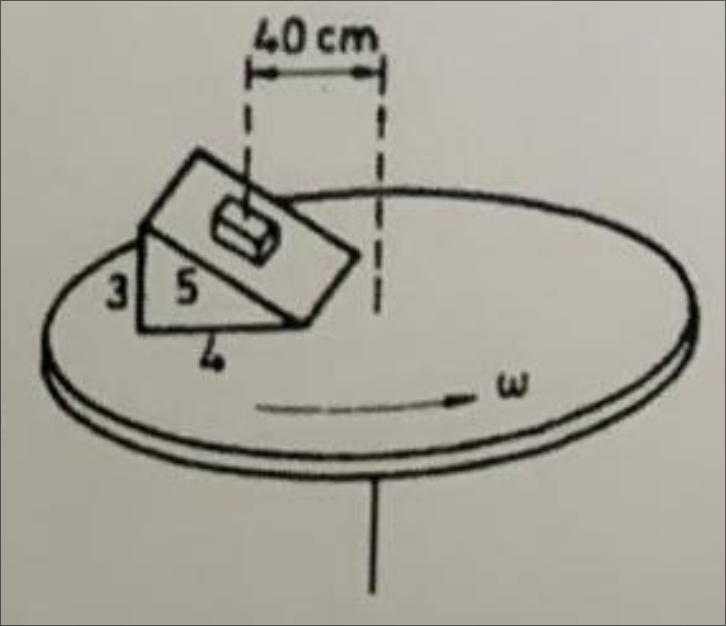
\includegraphics[width=.5\textwidth]{media/es_5_6.png}
    \end{center}
\end{figure*}

\subsection{5 Dicembre}

\subsection{11 Dicembre}

\sexercise{7.1}{
    Per ogni punto della traiettoria la pallina deve soddisfare la legge di Newton,
    affinché il giro della morte si completi, in particolare nel punto \(B\), dove
    la forza è data da
    \[
        mg + N - m\frac{v^2}{R} = 0
    \]
    Da cui ricaviamo la reazione vincolare
    \[
        N = m\frac{v^2}{R} - mg
    \]
    la reazione vincolare in \(B\) deve essere maggiore o uguale a zero, come condizione limite
    per completare il giro della morte.
    Quindi, \begin{align*}
        m\frac{v^2}{R} - mg &\geq 0 \\
        v^2 &\geq Rg
    \end{align*}
    Ora, leghiamo la velocità con l'altezza di partenza. Consideriamo
    la conservazione dell'energia. Nel punto iniziale l'energia è \(mgh\)
    e in \(B\) è \(\frac{1}{2} m v_b^2 + 2mgR\).
    Allora ricaviamo
    \[
        h = 2R + \frac{1}{2} \frac{v_b^2}{g}
    \]
    Il valore minimo è allora
    \[
        h \geq 2 E + \frac{1}{2}\frac{Rg}{g} = \frac{5}{2}R
    \]
    L'energia è iniziale è la medesima con la quale la molla viene schiacciata.
    Abbiamo allora
    \[
        mgh = \frac{1}{2} k x^2
    \]
    e quindi la compressione è data da
    \[
        x = \sqrt{\frac{2mgh}{k}} = \sqrt{\frac{5mgR}{k}}
    \]
}

\sexercise{7.2}{
    Vi sono la forza elastica, quella di gravità, e il vincolo
    della pallina sul piatot. La legge di Newton del piatto, fino a quanto stanno a contatto,
    abbiamo
    \[
        m'a = - m'g + -k x - N
    \]
    e quella della pallina
    \[
        ma = -mg + N
    \]
    Troviamo quindi
    \[
        \begin{cases}
            mm'a = -mm'g - kmx - mN \\
            mm'a = -mm'g + m'N
        \end{cases}
    \]
    da cui ricaviamo
    \[
        N = \frac{-kmX}{m+m'} = -\frac{kmX}{M}
    \]
    Calcoliamo la compressione iniziale per cui piatto e pallina superano quota zero.
    L'energia iniziale è solo quella potenziale della molla \(E_i = \frac{1}{2}k{(\Delta L)}^2\).
    Essa deve pari a quella finale, che deve essere sufficiente per almeno arrivare a quota zero con velocità nulla.
    \[
        \frac{1}{2} k {(\Delta L)}^2 = Mg\Delta L
    \]
    da cui
    \[
        \Delta L = \frac{2Mg}{k}
    \]
}

\sexercise{7.3}{
    Il corpo rimarrà fermo se \(T \leq F_{att} = \mu_s m g = 2\mu_s m g\).
    La tensione è data da
    \[
        T - mg\cos\theta - m\frac{v^2}{l} = 0
    \]
    che è l'equazione di Newton per la sferetta.
    La tensione è massima quando \(\theta = 0\), quindi
    \[
        T_{\text{max}} = mg + m\frac{v^2}{l}
    \]
    Chiamiamo \(v_\text{max}\) la velocità per \(\theta = 0\).
    L'energia iniziale è data da
    \[
        E_i = mg ( l - l\cos\theta_0)
    \]
    dove fissiamo lo zero al punto minimo.
    Abbiamo allora
    \[
        \frac{1}{2}m v_\text{max} = mg(l - l\cos\theta_0)
    \]
    Da cui ricaviamo
    \[
        v_\text{max}^2 = 2gl(1-\cos\theta_0)
    \]
    Allora la tensione massima è data da
    \begin{align*}
        T_\text{max} &= mg + m \frac{2gl(1-\cos\theta_0)}{l} \\
        &= 3 mg - 2 mg\cos\theta_0
    \end{align*}
    Tale forza deve essere minore o uguale a quella di attrito
    \begin{align*}
        3 mg - 2 mg\cos\theta_0 &\leq 2\mu_s mg \\
        \theta_0 \leq \arccos\left(\frac{3-2\mu_s}{2}\right)
    \end{align*}
}

\sexercise{7.4}{
    Il momento angolare è
    \[
        L_0 = mvR = m\omega R^2
    \]
    che è costante. In particolare \(L_0 = m\omega_1 R_1^2\).
    Allora,
    \[
        \omega(R) = w_1 {\left(\frac{R_1}{R}\right)}^2
    \]
    Quindi, la tensione della fune è pari a
    \begin{align*}
        T &= m\frac{v^2}{R} = m\omega^2 R = m\omega_1^2 {\left(\frac{R_1}{R}\right)}^4 R \\
        &= m\omega_1^2 R_1 {\left(\frac{R_1}{R}\right)}^3
    \end{align*}
    La tensione massima ci dà la condizione per il raggio minimo
    \[
        T_\text{max} = m\omega_1^2 R_1 {\left(\frac{R_1}{R_\text{min}}\right)}^3
    \]
    da cui ricaviamo
    \[
        R_\text{min} = {\left(\frac{m\omega_1^2R_1^4}{T_\text{max}}\right)}^{1/3}
    \]
    Per ciò che concerne il lavoro abbiamo
    \begin{align*}
        W &= \Delta E_K = \frac{1}{2} m v_2^2 - \frac{1}{2} m v_1^2 \\
        &=\frac{1}{2} m\omega_1^2 R_1^2 \left[
            {\left(\frac{R_1}{R_2}\right)}^2 - 1
        \right] 
    \end{align*}
    per il teorema dell'energia cinetica.
}

\sexercise{7.5}{
    Il momento nella direzione \(\hat{z}\) si conserva in quanto \(\vec{r} \wedge m\vec{g}\)
    è prtogonale all'asse \(z\).
    Abbiamo
    \[
        L_{0,az} = |\vec{r_A} \wedge m \vec{v_0}| = mv_0 R \sin\theta
    \]
    e
    \[
        L_{0, bz} =mvR
    \]
    Allora otteniamo la conservazione del momento angolare
    \[
        v = v_0\sin\theta
    \]
    L'energia è anche conservata.
    La condizione minima è che la velocità sia nulla in cima alla bacinella. In tal caso,
    la velocità verticale è nulla alla fine.
    \[
        \frac{1}{2} m v_0^2 + mgR(1 - \cos\theta) = \frac{1}{2} m v^2 + mgR
    \]
    e quindi
    \[
        v_0^2 = \frac{2gR}{\cos\theta}
    \]
}

\sexercise{7.6}{
    
}

\sexercise{7.7}{
    \[
        \integral[r][\infty][\frac{k}{r^3}][r]
    \]
}

\subsection{18 dicembre (urti)}

\sexercise{8.1}{
    Il volo dei proiettili è soggetto solo alla forza peso, e dopo l'urto
    il centro di massa delle due masse si muoverà di moto parabolico.
    Abbiamo quindi che
    \[
        m\frac{d\vec{V}_c}{dt} = m\vec{g}
    \]
    dove \(\vec{V}_c\) è la velocità del centro di massa. Possiamo allora scrivere
    \[
        \begin{cases}
            m\vec{a}_{cx} = 0 \\
            m\vec{a}_{cy} = - mg
        \end{cases}
        \implies \begin{cases}
            \vec{v}_{cx}(t) = v_0 \cos\alpha \\
            \vec{v}_{cy}(t) = v_0 \sin\alpha - gt \\
        \end{cases}
        \implies \begin{cases}
            \vec{x}_{cx}(t) = v_0 \cos\alpha t \\
            \vec{x}_{cy}(t) = v_0 \sin\alpha t - \frac{1}{2}gt^2
        \end{cases}
    \]
    Abbiamo allora
    \[
        y_{c} = x_{c} \tan\alpha = \frac{gx_c^2}{2v_0^2\cos^2alpha} = 0
    \]
    da cui troviamo la soluzione
    \[
        x_c = \frac{2v_0^2}{g} \cos\alpha\sin\alpha
    \]
    Questo punto del centro di massa è la media pesata dei due punti di atterraggio
    \[
        x_c \frac{x_1m_1 + x_2m_2}{m_1 + m_2}
    \]
    E quindi troviamo
    \[
        \frac{3}{2} x_c - \frac{x_2}{2}
    \]
}

\sexercise{8.2}{
    Abbiamo la conservazione
    \[
        \vec{p} = m_1\vec{v_{10}} + \frac{1}{2}m_1\vec{v_{20}} = 0
    \]
    Proiettando l'equazione della quantità di moto sull'asse delle ascisse troviamo
    \[
        p_x = m_1 v_{10} - \frac{1}{2}m_1 v_{20} = 0
    \]
    Il corpo \(1\) ha
    \[
        \begin{cases}
            a_x = 0 \\
            a_y = -g
        \end{cases}
        \implies
        \begin{cases}
            v_x = v_{10} \\
            v_y = -gt
        \end{cases}
        \implies
        \begin{cases}
            x_1 = v_{10} t \\
            y_1 = h - \frac{1}{2}gt^2
        \end{cases}
    \]
    Il momento in cui tocca terra è \(\overline{t} = \sqrt{\frac{2h}{g}}\)
    e quindi
    \[
        \overline{x_1} = x_1(\overline{t}) = v_{10} \sqrt{\frac{2h}{g}}
    \]
    Per il corpo \(2\) analogamente abbiamo
    \[
        \begin{cases}
            x_2 = v_{20} t \\
            y_2 = h - \frac{1}{2}gt^2
        \end{cases}
    \]
    quindi
    \[
        \overline{x_2} = x_2(\overline{t}) = -v_{20} \sqrt{\frac{2h}{g}}
        = - 2 v_{10} \sqrt{\frac{2h}{g}}
    \]
    La distanza è allora \[d = \overline{x_1} - \overline{x_2} = 3v_{10}\sqrt{\frac{2h}{g}}\]
    da cui ricaviamo \(v_{10}\) e \(v_{20}\).
}

\sexercise{8.3}{
    La distanza iniziale è \(L_0 - \Delta L\) e dopo che il filo viene tagliato
    le masse si cominciano a muovere con velocità \(v_1\) e \(v_2\).
    Visto che la forza della molla è interna, la quantità di moto lungo le ascisse si conserva.
    Quindi,
    \[
        p = -v_1v_1 + m_2v_2 = 0
    \]
    Allora
    \[
        |v_2| = \frac{m_1}{m_2} v_1 = \frac{v_1}{2}
    \]
    con direzione opposta.
    L'energia del sistema vale
    \begin{align*}
        \frac{1}{2} k \Delta L^2 &= \frac{1}{2} m_1 v_{1, \text{max}}^2 + \frac{1}{2} m_2 v_{2, \text{max}}^2 + 0 \\
        K\Delta L &= \frac{3}{2} m_1 v_{1,\text{max}}^2 \\
        v_{1,\text{max}} &= \sqrt{\frac{2}{3} \frac{k}{m_1}} \\
        v_{2,\text{max}} &= \sqrt{\frac{k}{6m_1}}
    \end{align*}
}

\sexercise{8.4}{
    Conservazione della quantità di moto
    \[
        \vec{p} + M\vec{v_1} + m\vec{v_2} = (M+m)\vec{v_1} + m\vec{v_{2,r}}
    \]
    la proiezione nell'ascisse è data da
    \[
        (M+m)v_1 - mv_{2,r} \cos\alpha = 0
    \]
    Da cui ricaviamo
    \[
        v_{2,r} = \frac{M+m}{m\cos\alpha} v_1
    \]
    Chiamiamo \(A = m\cos\alpha\).
    Dal teorema di Pitagora generalizzato
    \[
        v_2^2 = v_1^2 + v_{2,r}^2 - 2v_1 v_{2,r} \cos\alpha
    \]
    L'energia potenziale del cuneo non cambia quindi
    \begin{align*}
        mgh &= \frac{1}{2} Mv_1^2 + \frac{1}{2}mv_2^2 \\
        2gh &= \frac{v_1^2}{A} + \frac{v_1^2}{A^2\cos^2\alpha} - \frac{2v_1^2}{A} \\
        2gh &= v_1^2 \left(
            \frac{1}{A^2\cos^2\alpha} - \frac{1}{A}
        \right) \\
        v_1 &= \frac{\sqrt{2gh} A \cos\alpha}{\sqrt{1 - A^2\cos^2\alpha}}
    \end{align*}
}

\sexercise{8.5}{
    La quantità di moto e l'energia cinetica si conservano. Le velocità sono tutte parallele.
    Abbiamo allora
    \begin{align*}
        m_1v_0 &= m_1 v_1 + m_2 v_2 \\
        \frac{1}{2}m_1v_0^2 &= \frac{1}{2}m_1v_1^2 + \frac{1}{2}m_2v_2^2 \\
        v_1 &= \frac{m_1v_0 - m_2v_2}{m_1} \\
        m_1v_0^2 &= m_1 \left(
            v_0^2 + {\left(\frac{m_2}{m_1}\right)}^2 v_2^2 - 2 \frac{m_2}{m_1}v_2v_0
        \right) + m_2v_2^2 \\
        0 &= v_2 \left[\frac{m_1 + m_2}{m_1} v_2 - 2v_0\right] \\
        v_2 &= \frac{2m_1v_0}{m_1 + m_2} = \frac{v_0}{2} \\
        v_1 &= \frac{m_1 - m_2}{m_1 + m_2} v_0 = -\frac{v_0}{2}
    \end{align*}
    La traiettoria è data da
    \[
        y = h-\frac{gx^2}{2v_2^2}
    \]
    che deve essere nulla quando \(x=d\), da cui
    \[
        v_2 = \sqrt{\frac{g}{2h}} d
    \]
    e quindi
    \[
        v_0 = \sqrt{\frac{2g}{h}} d
    \]
}

\sexercise{8.6}{
    L'energia iniziale è
    \[
        E_1 = \frac{1}{2} kh^2
    \]
    appena prima di colpire \(m_2\) abbiamo
    \[
        E_2 = \frac{1}{2} m_1v_0^2 + \frac{1}{2} k \Delta L^2
    \]
    con \(\Delta L = d-L_0\). Abbiamo quindi \(E_1 = E_2\)
    per la conservazione dell'energia da cui
    \[
    v_0 = \sqrt{\frac{k}{m_1} (h^2 - \Delta L^2)}
    \]
    L'urto è elastico e centtale quindi
    \[
        v_1 = \frac{m_1 - m_2}{m_1 + m_2} v_0 = - \frac{v_0}{2}
    \]
    Quindi l'energia subito dopo l'urto è
    \begin{align*}
        E_3 &= \frac{1}{2} m_1v_1^2 + \frac{1}{2} k \Delta L^2\\
        &= \frac{1}{8}m_1v_0^2 + \frac{1}{2}k\Delta L^2 \\
        &= \frac{1}{2} k \left(\frac{1}{4}h^2 + \frac{3}{4}\Delta L^2\right)
    \end{align*}
    Calcoliamo allora la massima compressione,
    quindi
    \begin{align*}
        E_4 &= \frac{1}{2} k \Delta L_{\text{max}}^2 = E_3 \\
        L_{\text{max}} &= \frac{1}{4}h^2 + \frac{3}{4} {d-L_0}^2
    \end{align*}
}

\sexercise{8.7}{
    XXX
}

\end{document}